%%%%%%%%%%%%%%%%%%%%%%%%%%%%%%%%%%%%%%%%%
% Short Sectioned Assignment LaTeX Template Version 1.0 (5/5/12)
% This template has been downloaded from: http://www.LaTeXTemplates.com
% Original author:  Frits Wenneker (http://www.howtotex.com)
% License: CC BY-NC-SA 3.0 (http://creativecommons.org/licenses/by-nc-sa/3.0/)
%%%%%%%%%%%%%%%%%%%%%%%%%%%%%%%%%%%%%%%%%

%----------------------------------------------------------------------------------------
%	PACKAGES AND OTHER DOCUMENT CONFIGURATIONS
%----------------------------------------------------------------------------------------

\documentclass[paper=a4, fontsize=11pt]{scrartcl} % A4 paper and 11pt font size

% ---- Entrada y salida de texto -----

\usepackage[T1]{fontenc} % Use 8-bit encoding that has 256 glyphs
\usepackage[utf8]{inputenc}

% ---- Idioma --------

\usepackage[spanish, es-tabla]{babel} % Selecciona el español para palabras introducidas automáticamente, p.ej. "septiembre" en la fecha y especifica que se use la palabra Tabla en vez de Cuadro

% ---- Otros paquetes ----

\usepackage{amsmath,amsfonts,amsthm} % Math packages
\usepackage{graphics,graphicx, floatrow} %para incluir imágenes y notas en las imágenes
\usepackage{graphics,graphicx, float} %para incluir imágenes y colocarlas
\usepackage{hyperref} % url in references

% Para hacer tablas comlejas
\usepackage{multirow}
\usepackage{threeparttable}

\usepackage{fancyhdr} % Custom headers and footers
\pagestyle{fancyplain} % Makes all pages in the document conform to the custom headers and footers
\fancyhead{} % No page header - if you want one, create it in the same way as the footers below
\fancyfoot[L]{} % Empty left footer
\fancyfoot[C]{} % Empty center footer
\fancyfoot[R]{\thepage} % Page numbering for right footer
\renewcommand{\headrulewidth}{0pt} % Remove header underlines
\renewcommand{\footrulewidth}{0pt} % Remove footer underlines
\setlength{\headheight}{13.6pt} % Customize the height of the header

\numberwithin{equation}{section} % Number equations within sections (i.e. 1.1, 1.2, 2.1, 2.2 instead of 1, 2, 3, 4)
\numberwithin{figure}{section} % Number figures within sections (i.e. 1.1, 1.2, 2.1, 2.2 instead of 1, 2, 3, 4)
\numberwithin{table}{section} % Number tables within sections (i.e. 1.1, 1.2, 2.1, 2.2 instead of 1, 2, 3, 4)

\setlength\parindent{0pt} % Removes all indentation from paragraphs - comment this line for an assignment with lots of text

\newcommand{\horrule}[1]{\rule{\linewidth}{#1}} % Create horizontal rule command with 1 argument of height
\usepackage{textcomp}
\usepackage{listings}
\usepackage{color}

\definecolor{mygreen}{rgb}{0,0.6,0}
\definecolor{mygray}{rgb}{0.5,0.5,0.5}
\definecolor{mymauve}{rgb}{0.58,0,0.82}

\lstset{ %
  backgroundcolor=\color{white},   % choose the background color; you must add \usepackage{color} or \usepackage{xcolor}; should come as last argument
  breakatwhitespace=false,         % sets if automatic breaks should only happen at whitespace
  breaklines=true,                 % sets automatic line breaking
  captionpos=b,                    % sets the caption-position to bottom
  commentstyle=\color{mygreen},    % comment style
  deletekeywords={...},            % if you want to delete keywords from the given language
  escapeinside={\%*}{*)},          % if you want to add LaTeX within your code
  extendedchars=true,              % lets you use non-ASCII characters; for 8-bits encodings only, does not work with UTF-8
  frame=single,	                   % adds a frame around the code
  keepspaces=true,                 % keeps spaces in text, useful for keeping indentation of code (possibly needs columns=flexible)
  keywordstyle=\color{blue},       % keyword style
  language=C,                 % the language of the code
  morekeywords={*,...},            % if you want to add more keywords to the set
  numbers=left,                    % where to put the line-numbers; possible values are (none, left, right)
  numbersep=5pt,                   % how far the line-numbers are from the code
  numberstyle=\tiny\color{mygray}, % the style that is used for the line-numbers
  rulecolor=\color{black},         % if not set, the frame-color may be changed on line-breaks within not-black text (e.g. comments (green here))
  showspaces=false,                % show spaces everywhere adding particular underscores; it overrides 'showstringspaces'
  showstringspaces=false,          % underline spaces within strings only
  showtabs=false,                  % show tabs within strings adding particular underscores
  stringstyle=\color{mymauve},     % string literal style
  tabsize=2,	                   % sets default tabsize to 2 spaces
}

\usepackage[table,xcdraw]{xcolor}


\newpage         


%----------------------------------------------------------------------------------------
%	INDICE
%----------------------------------------------------------------------------------------

\begin{document}
	
\setcounter{page}{0}

\begin{titlepage}
 
 
\newlength{\centeroffset}
\setlength{\centeroffset}{-0.5\oddsidemargin}
\addtolength{\centeroffset}{0.5\evensidemargin}
\thispagestyle{empty}

\noindent\hspace*{\centeroffset}\begin{minipage}{\textwidth}

\centering

\includegraphics[width=0.9\textwidth]{images/logo_ugr.jpg}\\[1.4cm]

\textsc{ \Large CLOUD COMPUTING: SERVICIOS Y APLICACIONES\\[0.2cm]}
\textsc{ MÁSTER EN INGENIERÍA INFORMÁTICA }\\[1cm]
% Upper part of the page
% 
% Title
{\Huge\bfseries Computación	Distribuida	y	Escalable	con	Hadoop	}
\noindent\rule[-1ex]{\textwidth}{3pt}\\[3.5ex]
{\large\bfseries Práctica 4}
\end{minipage}

\vspace{4.5cm}
\noindent\hspace*{\centeroffset}\begin{minipage}{\textwidth}
\centering

\textbf{Autor}\\ {Juan Pablo Porcel Porcel - juanpiporcel@correo.ugr.es}\\[1cm]

\includegraphics[width=0.3\textwidth]{images/etsiit_logo.png}\\[0.1cm]
\textsc{Escuela Técnica Superior de Ingenierías Informática y de Telecomunicación}\\
\textsc{---}\\
Granada, 22 de mayo de 2017
\end{minipage}
%\addtolength{\textwidth}{\centeroffset}
%\vspace{\stretch{2}}
\end{titlepage}




\thispagestyle{empty}

\newpage %inserta un salto de página

\tableofcontents % para generar el índice de contenidos

%\listoffigures

\newpage

%----------------------------------------------------------------------------------------
%	DOCUMENTO
%----------------------------------------------------------------------------------------

\section{Introducción}

El objetivo de esta práctica es familiarizarse con el uso de una plataforma PaaS y desarrollar habilidades de despliegue de contenedores y configurar aplicaciones sencillas en los mismos. \\

Para ello el alumno deberá realizar las tareas que se describen a continuación y entregar documentación describiendo con el mayor detalle posible todas las actividades realizadas. \\

\begin{itemize}
	\item Crear un contenedor docker con un servidor web con SSL.
	\begin{enumerate}
		\item ¿Cuál es el puerto SSL?
		\item ¿Cómo redirigir el puerto SSL a vuestro puerto asignado?
	\end{enumerate}
	\item Crear una página en el servidor web que se conecte a un servicio de base de datos en otro contenedor.
	\item Duplicar los contenedores y discutir o mostrar qué pasaría si uno de ellos cayese.
	\item Desplegar un servicio OwnCloud o NewCloud en otro contenedor y chequear su correcto funcionamiento almacenando archivos.
	\item Elaborar un breve documento detallando el trabajo realizado.
\end{itemize}


\section{Configuración de los contenedores docker}

Para esta práctica se han creado tres contenedores docker para desplegar la aplicación web creada para la primera práctica. En la Figura \ref{fig:} se puede ver un esquema de la conexión entre los tres contenedores. \\

\begin{figure}[h!]
	\centering
	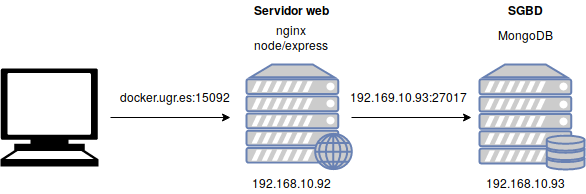
\includegraphics[width=13cm]{./images/ccsa}
	\caption{Conexión entre los contenedores.} 
	\label{fig:ccsa}
\end{figure}

El despliegue de la aplicación se puede llevar a cabo con docker-compose o siguiendo los pasos que se detallan en las siguientes subsecciones para trabajar sólamente con Docker. \\

El archivo de configuración para docker-compose se muestra a continuación. \\

\begin{lstlisting}
version: '3'

services:
  jpblo_nginx:
    build:
      context: ./nginx
      dockerfile: Dockerfile
    container_name: jpblo_nginx
    ports:
      - "14080:80"
      - "14083:443"
    links:
      - "jpblo_app:app"

  jpblo_app:
    build:
      context: ./app
      dockerfile: Dockerfile
    container_name: jpblo_app
    ports:
      - "14082:8080"
    links:
      - "jpblo_mongo:mongodb"

  jpblo_mongo:
    image: mongo
    container_name: jpblo_mongo
    ports:
      - "14081:27017"
      
  mongo-seed:
    build: ./mongo
    links:
      - "jpblo_mongo:mongodb"
\end{lstlisting}

Mediante este fichero de configuración se han especificado la redirección de puertos para cada contenedor y la conexión entre ellos mediante la etiqueta \textbf{links}. Los ficheros dockerfile de configuración para los dos primeros contenedores se detallan más adelante. El contenedor mongo-seed se usa para cargar en el contenedor con el sistema gestor de base de datos la base de datos de prueba. \\

\subsection{SGBD}

Antes de nada vamos a clonar el repositorio de la asignatura con la aplicación web y los archivos de configuración y provisionamiento. \\

\begin{lstlisting}
git clone https://github.com/JPPorcel/CCSA.git ./app
\end{lstlisting}

El primer contenedor tendrá alojado un sistema gestor de base de datos. Para desplegar este contenedor se ha elegido la imagen de \textbf{mvertes/alpine-mongo} alojada en \href{https://hub.docker.com/r/mvertes/alpine-mongo/}{DockerHub} debido a que la versión oficial de mongo producía un error al desplegar el contenedor en \textit{hadoop.ugr.es}. Podemos crear el contenedor con el siguiente comando: \\

\begin{lstlisting}
docker run -d -p 14081:27017 --name jpblo_mongo mvertes/alpine-mongo
\end{lstlisting}

Una vez que el contenedor esté corriendo podemos conectarnos a la base de datos mongo para comprobar que todo ha ido bien con: \\

\begin{lstlisting}
docker exec -i -t jpblo_mongo mongo
\end{lstlisting}

Ahora vamos a importar la base de datos de prueba a el contenedor con \textbf{mongoimport}. Tenemos que conectarnos por el puerto que hemos especificado en docker (14081). El archivo restaurantes.json se encuentra en la ruta P2/mongo/ dentro del repositorio. \\

\begin{lstlisting}
mongoimport --host 127.0.0.1 --port 14081 --db restaurants --collection restaurants --drop --file restaurantes.json
\end{lstlisting}

\subsection{Aplicación Web}

Ahora vamos a desplegar el contenedor con la aplicación web. Para ello usaremos el \textbf{Dockerfile} que se encuentra en P2/app/: \\

\begin{lstlisting}
FROM keymetrics/pm2-docker-alpine

# Create app directory
RUN mkdir -p /opt/app
WORKDIR /opt/app

# Install app dependencies
COPY package.json /opt/app/
RUN npm install

# Bundle app source
COPY . /opt/app

EXPOSE 8080

CMD pm2 start --no-daemon server.js
\end{lstlisting}

La imagen base para este contenedor es \textbf{keymetrics/pm2-docker-alpine} que tiene ya instalado NodeJS y pm2 para administrar la aplicación. Mediante este dockerfile añadimos los fuentes de la aplicación y exponemos el puerto 8080 que será el puerto de escucha de la aplicación. Por último lanzamos la aplicación con $pm2 start --no-daemon server.js$. \\

Desde el mismo directorio donde se encuentra este dockerfile podemos contruir la imagen con: \\

\begin{lstlisting}
cd app/P2/app && docker build -t jpblo/webapp .
\end{lstlisting}

Y lanzarlo especificando la redirección del puerto 8080 a uno de los puertos disponibles y especificando el nombre del host donde se encuentra la base de datos mongo \textbf{jpblo\_mongo:mongodb}: \\

\begin{lstlisting}
docker run -d --link jpblo_mongo:mongodb -p 14082:8080 --name jpblo_app jpblo/webapp
\end{lstlisting}

\subsection{Servidor Web}

Para desplegar el contenedor con el servidor web \textbf{nginx} usaremos el siguiente Dockerfile que se encuentra en la ruta P2/nginx/ dentro del repositorio. \\

\begin{lstlisting}
FROM nginx

# Copy custom configuration file from the current directory
COPY nginx.conf /etc/nginx/nginx.conf
\end{lstlisting}

Este dockerfile carga la imagen oficial de nginx y añade el archivo de configuración de nginx al contenedor. \\

\begin{lstlisting}
worker_processes auto;

events { worker_connections 1024; }

http {
	server {
			listen 80;
		
			location / {
			proxy_pass http://app:8080;
			proxy_http_version 1.1;
			proxy_set_header Upgrade $http_upgrade;
			proxy_set_header Connection 'upgrade';
			proxy_set_header Host $host;
			proxy_cache_bypass $http_upgrade;
			}
	}
}
\end{lstlisting}

Podemos contruir la imagen para este contenedor con: \\

\begin{lstlisting}
cd app/P2/nginx && docker build -t jpblo/nginx .
\end{lstlisting}

Y lanzarlo especificando de nueco la redirección del puerto 80 a uno de los puertos disponibles, así como el puerto SSL (\textbf{14083:443}), y el nombre del host donde se encuentra la aplicación web \textbf{jpblo\_app:app}: \\

\begin{lstlisting}
docker run -d --link jpblo_app:app -p 14080:80 -p 14083:443 --name jpblo_nginx jpblo/nginx
\end{lstlisting}

El servidor web nginx escuchará en el puerto 80 y redireccionará las peticiones a donde se encuentra nuestra aplicación corriendo \textbf{app:8080}. \\

Con nginx también podemos realizar un balanceo de carga replicando los contenedores que contienen la aplicación y añadiendo sus direcciones al archivo de configuración de nginx. Un ejemplo podría ser el que se muestra en el siguiente fichero de configuración de nginx con tres contenedores con la aplicación replicados. \\


\begin{lstlisting}
worker_processes 4;

events { worker_connections 1024; }

http {
	upstream node-app {
		least_conn;
		server node1:8080 weight=10 max_fails=3 fail_timeout=30s;
		server node2:8080 weight=10 max_fails=3 fail_timeout=30s;
		server node3:8080 weight=10 max_fails=3 fail_timeout=30s;
	}
		
	server {
		listen 80;
	
		location / {
			proxy_pass http://node-app;
			proxy_http_version 1.1;
			proxy_set_header Upgrade $http_upgrade;
			proxy_set_header Connection 'upgrade';
			proxy_set_header Host $host;
			proxy_cache_bypass $http_upgrade;
		}
	}
}
\end{lstlisting}

De esta manera conseguimos que el trabajo esté repartido entre los tres contenedores y que si falla alguno no deje de estar la aplicación inoperativa. \\

\begin{figure}[h!]
	\centering
	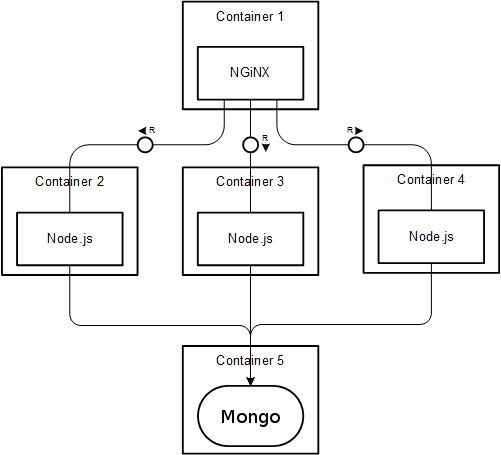
\includegraphics[width=13cm]{./images/balanced}
	\caption{Aplicación web replicada en tres contenedores} 
	\label{fig:balanced}
\end{figure}

\section{Aplicación web}

En la Figura \ref{fig:app} se puede ver una captura del servidor corriendo en la dirección \href{hadoop.ugr.es:14080}{hadoop.ugr.es:14080}. \\

\begin{figure}[h!]
	\centering
	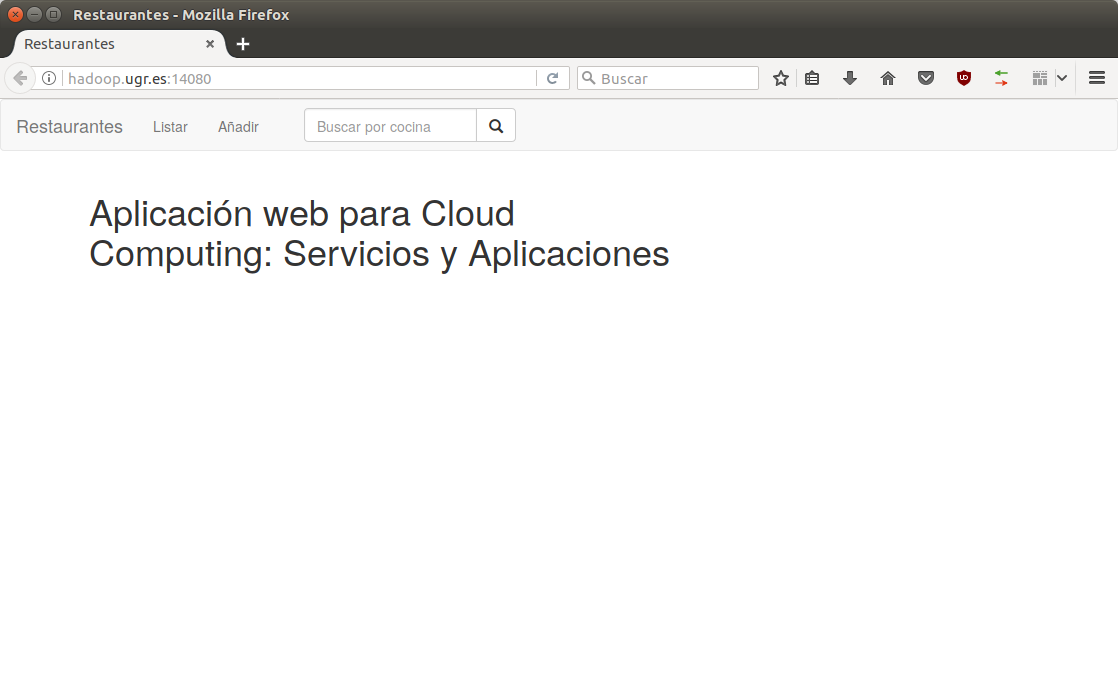
\includegraphics[width=13cm]{./images/running}
	\caption{Aplicación web corriendo en hadoop.ugr.es:14080} 
	\label{fig:app}
\end{figure}

La aplicación está escrita en NodeJS con Express y Pug y usa una base de datos Mongo para almacenar la información. Es una aplicación muy sencilla. Se trata de un gestor de restaurantes donde se pueden añadir nuevos restaurante desde la opción de añadir que nos mostrará un formulario como el de la Figura \ref{fig:nuevo}. \\

\begin{figure}[h!]
	\centering
	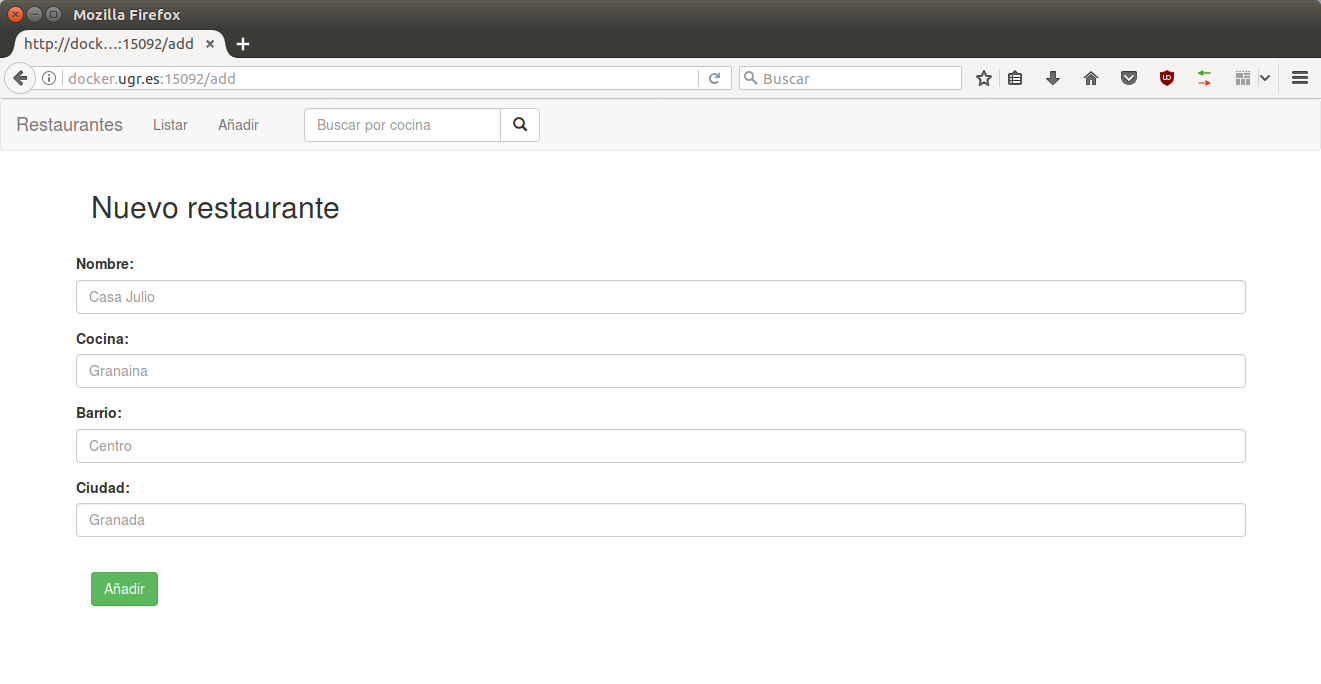
\includegraphics[width=13cm]{./images/nuevo}
	\caption{Formulario para añadir un nuevo restaurante} 
	\label{fig:nuevo}
\end{figure}

En la sección de Listar nos aparecen los primeros 20 restaurantes de la base de datos. Podemos filtrar los restaurantes por nombre, ciudad o tipo de cocina. El buscador que se encuentra implementado en la página buscará por tipo de cocina pero se pueden añadir más parámetros en la url, por ejemplo \textit{cocina=Granaina\&nombre=Julio\&ciudad=Granada}. En las Figura \ref{fig:buscar} y Figura \ref{fig:consultar} vemos la búsqueda y consulta de un restaurante añadido a la base de datos. \\

\begin{figure}[h!]
	\centering
	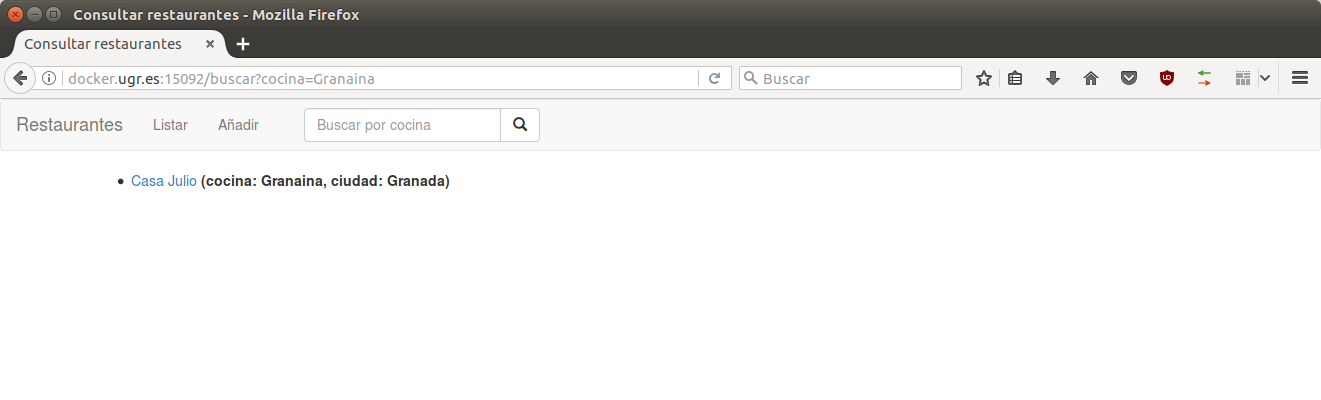
\includegraphics[width=13cm]{./images/buscar}
	\caption{Buscar un restaurante} 
	\label{fig:buscar}
\end{figure}

\begin{figure}[h!]
	\centering
	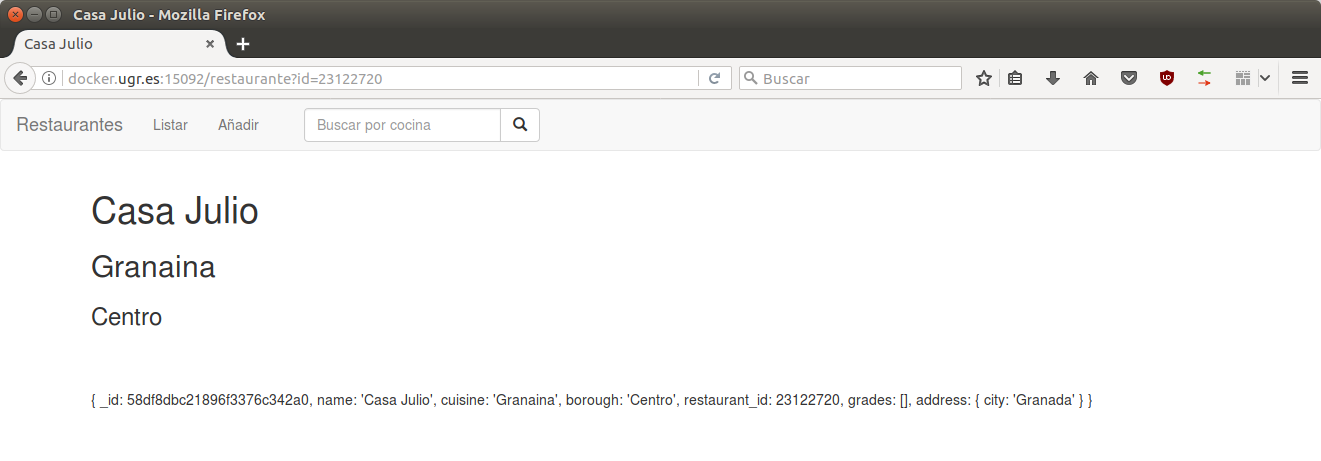
\includegraphics[width=13cm]{./images/consultar}
	\caption{Consultar un restaurante} 
	\label{fig:consultar}
\end{figure}

\section{OwnCloud}

Para poner en marcha OwnCloud en hadoop.ugr.es con docker usaremos dos contenedores. El primero contendrá la aplicación de OwnCloud y el segundo alojará una base de datos PostgreSQL para conseguir persistencia en los datos de la aplicación, como las cuentas de usuario y los índices a los archivos. \\

Podemos desplegar ambos contenedores con: \\

\begin{lstlisting}
docker run -d --name jpblo_postgres -e POSTGRES_PASSWORD=password postgres
docker run -d -p 14084:80 --name jpblo_owncloud --link jpblo_postgres:owncloud-db owncloud
\end{lstlisting}

Ahora podemos acceder a \url{hadoop.ugr.es:14084} y configurar el usuario administrador de OwnCloud y la base de datos que se va a utilizar como aparece en la Figura \ref{fig:owncloud}. \\

\begin{figure}[h!]
	\centering
	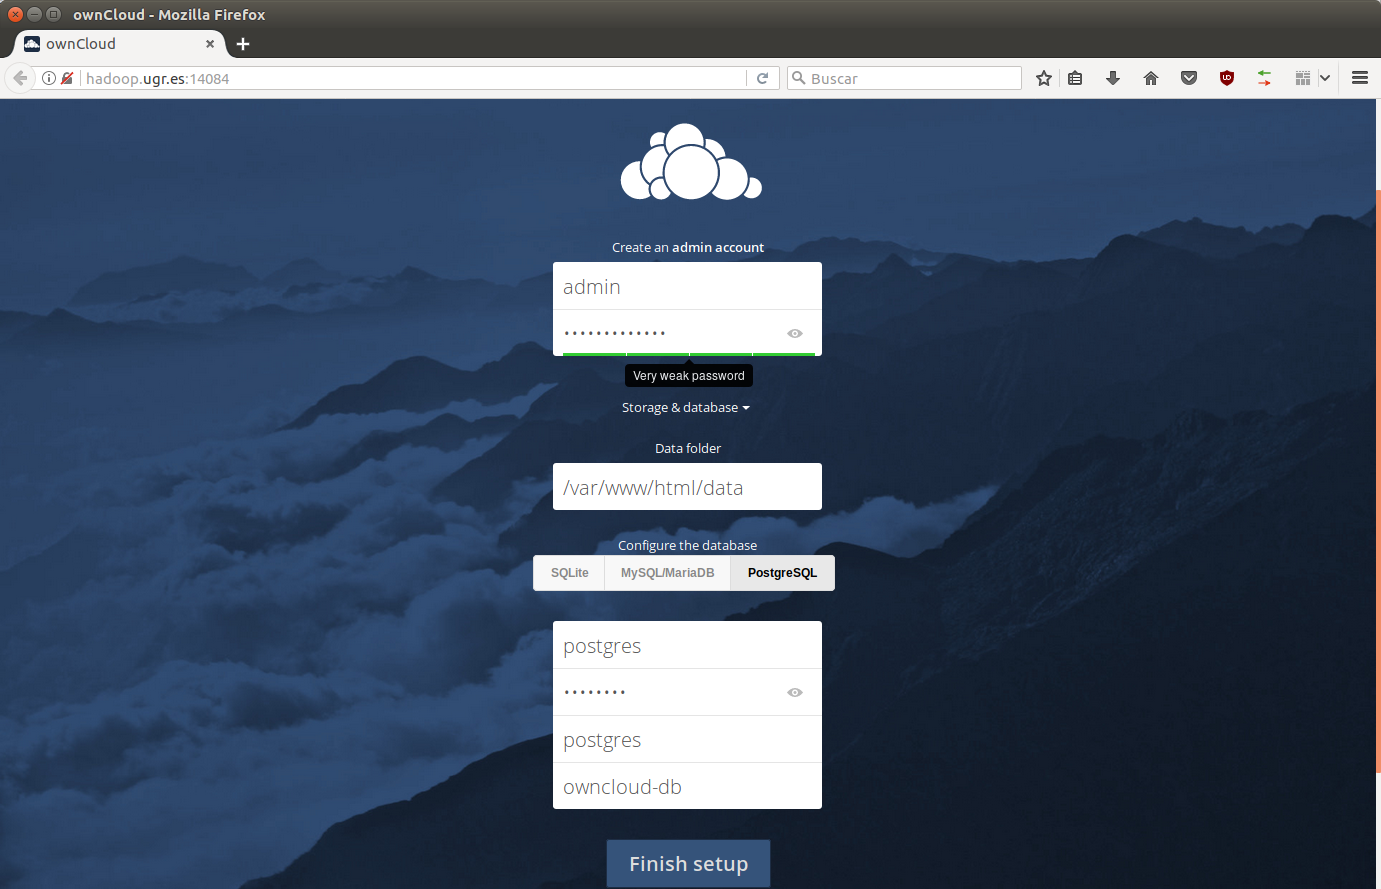
\includegraphics[width=13cm]{./images/owncloud}
	\caption{Configuración de la base de datos PostgreSQL en OwnCloud} 
	\label{fig:owncloud}
\end{figure}


\begin{figure}[h!]
	\centering
	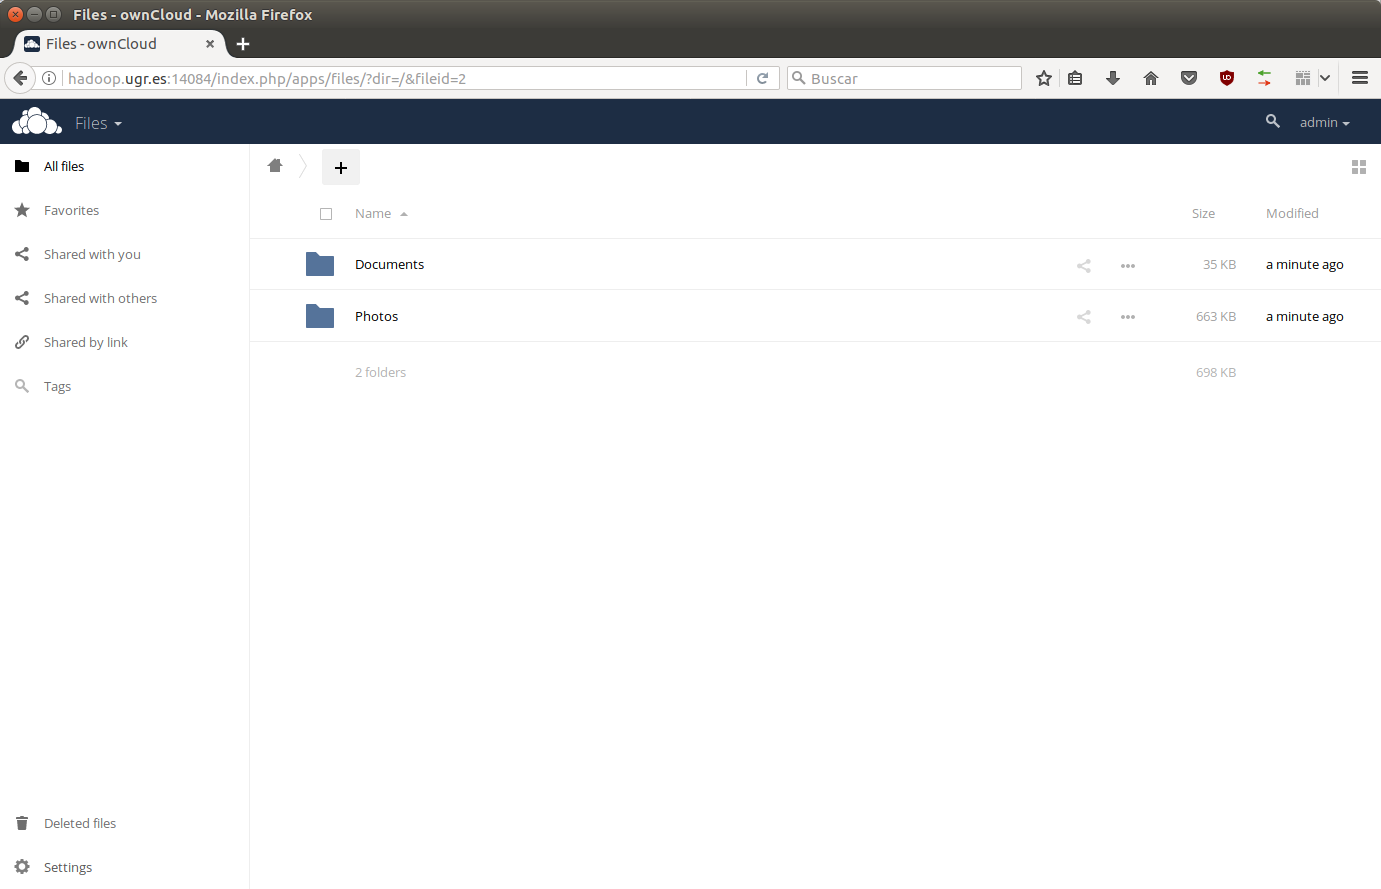
\includegraphics[width=13cm]{./images/owncloud2}
	\caption{Aplicación OwnCloud corriendo en hadoop.ugr.es:14084} 
	\label{fig:owncloud2}
\end{figure}



\section{Conclusiones}

Mediante esta práctica se ha intentado familiarizar al alumno con el uso de una plataforma PaaS. Al contrario de la primera práctica, en esta segunda práctica no se han tenido problemas de conexión con la plataforma y se ha podido realizar la práctica correctamente. \\

El uso de contenedores es una tecnología muy usada hoy en día para el despliegue de aplicaciones web ya que conseguimos abstraernos del sistema operativo donde se ejecutará la aplicación quitándonos problemas de compatibilidad y provisionamiento. También, cabe destacar que el balanceo de carga es mucho más sencillo llevarlo a cabo con contenedores que con máquinas virtuales. \\



\end{document}
